\chapter{معرفی \ws{rl}}\label{ch:rl}
\section{مقدمه}
\subsection{جایگاه \ws{rl} در \ws{ml}}
بسیاری از صاحب نظران \w{ml} را به سه دسته تقسیم می‌کنند :
\begin{enuminline}
	\item \w{supLearning}
	\item \w{unsupLearning} یا \w{clustering}
	\item \w{semisupLearning}
\end{enuminline}

در این میان،
\w{rl}
را بعضی ها دسته چهارم می‌دانند و  بعضی دیگر آن‌را در دسته سوم قرار می‌دهند. بر اساس دسته‌بندی گروه دوم شکل 
\ref{fig:rl-machinelearning-chart}
رسم شده است.


همچنین شکل 
\ref{fig:rl-chart}
کابرد \w{rl} را در علوم مختلف نشان می‌دهد.

\begin{figure}[h!]
	\centering
	\def\localheigth{7cm}
	\subfigure[]{%
		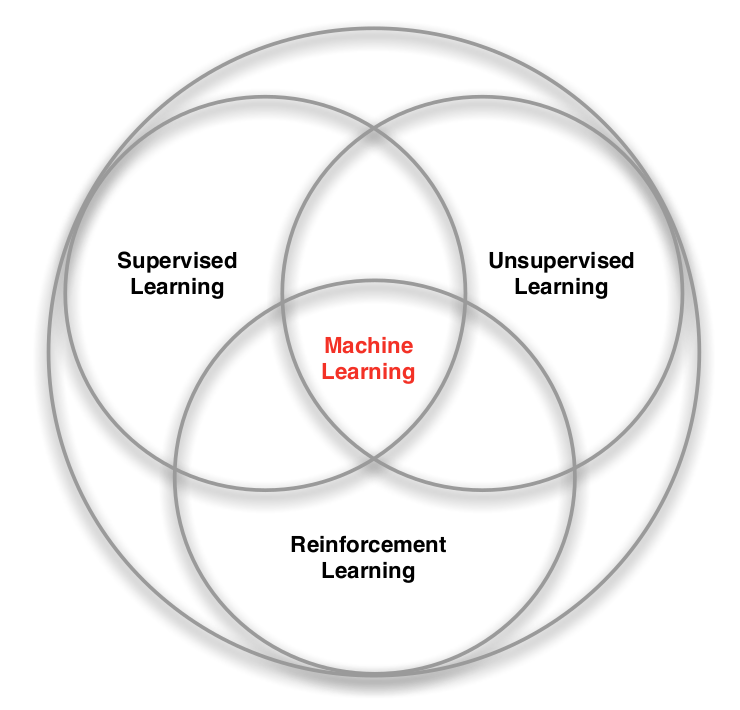
\includegraphics[height=\localheigth]{Figures/RL/RL-machinelearning-chart}
		\label{fig:rl-machinelearning-chart}
	}
	%  	\hspace*{1.5cm} % space between two figures
	\subfigure[جایگاه \lr{RL} در علوم مختلف]{%
		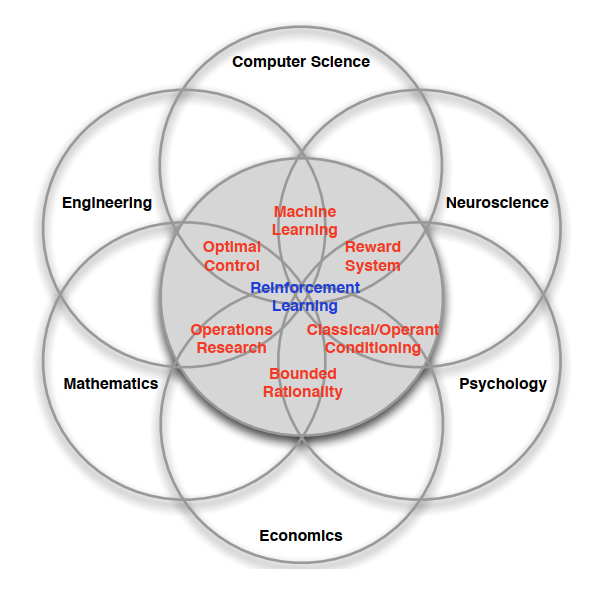
\includegraphics[height=\localheigth]{Figures/RL/RL-chart}
		\label{fig:rl-chart}
	}
	\caption{%
		جایگاه \ws{rl}
	}
	\label{fig:Rl-circle-total}
\end{figure}



\subsection[وجه تمایز 
\ws{rl}
از دیگر الگو‌های 
\ws{ml}
]{چه چیزی 
\ws{rl}
را با دیگر الگوهای 
\ws{ml}
متمایز می‌کند؟
}

این سوال از آن جهت حایز اهمیت است که بیان می‌کند چرا ما به سراغ الگوی 
\w{rl}
رفته‌ایم. پاسخ ملاحظات زیر است.

\begin{alphabetlist}
\item هیچ 
\w{sup}
وجود ندارد و صرفا \w{reward}ها وجود دارند.
\item 
\w{feedback}
همراه با تاخیر است وبه صورت همزمان رخ نمی‌دهد.
\RTLfootnote{در مورد علت تاخیر در ادامه توضیح داده خواهد شد.}
\item 
مفهوم زمان واقعا مطرح است و یک ترتیب خاص از داده ها داریم.
شکل \ref{fig:markov-chain-sarsa} این توالی زمانی را نشان می‌دهد.
\end{alphabetlist}

\w{rl}(\gls{a:rl})
بر اساس \w{rewardhypo} پایه‌گذاری می‌شود.
\begin{definition}[\w{rewardhypo}]
	همه اهداف می‌توانند براساس بیشینه کردن مقدار میانگین تجمعی امتیازها توصیف کرد.
\end{definition}

ممکن است این عبارت کمی عجیب بنظر برسد اما در بسیاری از مسایل که به صورت برد و باخت و به نوعی دو حالت مطلوب و نامطلوب دارند، می‌توان در ساده ترین حالت مقدار $+1$ را برای برد و $-1$ را برای باخت در نظر گرفت.

\begin{remark}
	در برخی منابع بجای \w{reward} از مفهوم \w{cost} استفاده می‌کنند و هدف الگوریتم آن می‌شود که به سمتی حرکت کند که کمترین \w{cost} را داشته باشد. برای یک‌پارچه‌سازی این مفاهیم معمولا یک علامت منفی برای این دو در نظر میگیرند یعنی :
	\[	\text{\rl{\w{reward}}} = -\text{\rl{\w{cost}}}
		\quad \colon \quad
		r = -c
		\]
\end{remark}

\subsection{
\ws{agent} و \ws{env}
}
 
 این مفهوم بسیار مفهوم مهمی می‌باشد و بارها از آن در این پروژه یاد شده است.
 
 در مسایل \w{rl} یک 
 \textbf{\w{agent}}
 وحود دارد که در یک \textbf{\w{env}} درحال تعامل است. \w{env} می‌تواند محیط اطراف \w{agent} باشد و یا هرچیزی که \w{agent} با آن در تعامل است.
  \cite{uclRL}
\begin{figure}[t]
	\centering
	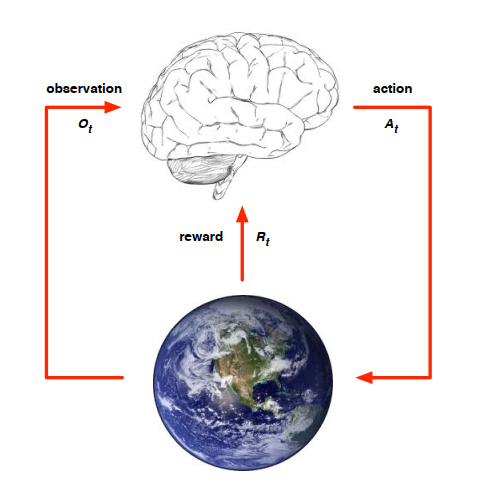
\includegraphics[width=0.7\linewidth]{Figures/RL/Enviroment-brain-as-agent}
	\caption{}
	\label{fig:enviroment-brain-as-agent}
\end{figure}

این تعامل به این صورت است که \w{agent} که در ابتدا یک \w{state} اولیه دارد، یک \w{action} بر روی \w{env} در زمان $t$ انجام می‌دهد. 
\w{env} مقدار \w{action} در زمان $t$ را دریافت می‌کند و 
سپس \w{env} در زمان $t+1$ دو اطلاعات مهم را بر می‌گرداند. 
\begin{alphinline}
	\item \w{obs}
	\item \w{reward}
\end{alphinline}

شکل 
\ref{fig:enviroment-brain-as-agent}
و \ref{fig:markov-chain-sarsa}
این تعامل را نشان می‌دهد. لازم به ذکر است که در پایان هر \w{step} مقدار $t$ یک واحد افزایش می‌یابد.

\subsection{\ws{state}}
در بخش قبل تعریف مناسبی از \w{state} ارایه نشد. برای این تعریف ابتدا مفهوم \w{history} ارایه می‌شود و از روی آن \w{state} تعریف خواهد شد.

\begin{definition}[\w{history}]
	به سری شامل \w{obs}، \w{action} و \w{reward} می‌باشد:
	\[
	\mathcal{H}_t = \mathcal{O}_1 ,\mathcal{R}_1, \mathcal{A}_1, \dots, \mathcal{A}_{t-1}, \mathcal{O}_{t-1}, \mathcal{R}_t
	\]
\end{definition}


\begin{figure}[t]
	\centering
	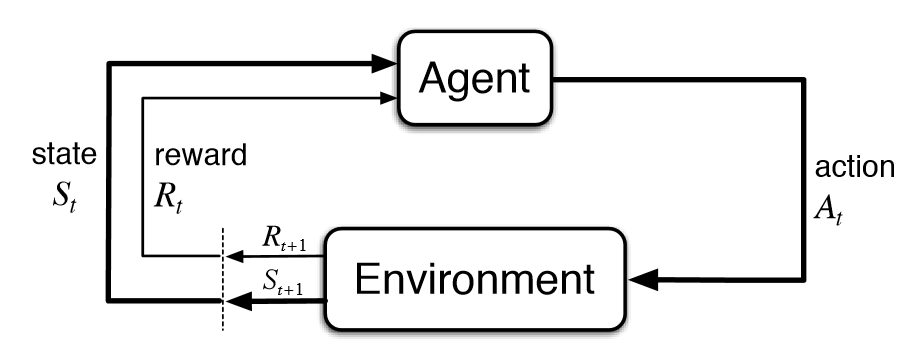
\includegraphics[width=0.7\linewidth]{Figures/RL/Markov-vhain-SARSA}
	\caption{شماتیک تعامل محیط با عامل}
	\label{fig:markov-chain-sarsa}
\end{figure}

با این تعریف \w{state} را می‌توان به شکل زیر تعریف کرد.

\begin{definition}\label{def:state}
	\textbf{\w{state}}
	اطلاعاتی است که در محاسبات برای آن‌که در بعد چه اتفاقی بیافتد، استفاده می‌شود. به عبارت دیگر \w{state} تابعی از \w{history} می‌باشد.
	\[
	\mathcal{S}_t = f(\mathcal{H}_t)
	\]
\end{definition}

دو نوع \w{state} وجود دارد.
\begin{alphabetlist}
	\item \textbf{\w{env state}} که با علامت $S_t^e$ نشان داده می‌شود.
	اطلاعات نهان \w{env} را نشان می‌دهد و معمولا برای \w{agent} به‌طور کامل دیده نمی‌شود. حتی اگر برای \w{agent} مشاهده‌پذیر نیز باشد، ممکن است اطلاعات کاملا بی‌ربطی را همراه داشته باشد.
	\item \textbf{\w{agent state}} که با علامت $S_t^a$ نشان داده می‌شود.
	که برابر است با هر اطلاعاتی که \w{agent} برای رسیدن به \w{action} بعدی با استفاده از الگوریتم های \gls{a:rl} استفاده می‌کند. 
\end{alphabetlist}

بنابراین در نعریف \ref{def:state} مناسب‌تر است بجای واژه \w{state} از \w{agent state} استفاده شود. بنابراین:
	\[
	\mathcal{S}_t^a = f(\mathcal{H}_t)
	\]
	
\begin{note}
	از این پس در سراسر این پایان‌نامه هرجا صحبت از \w{state} شد منظور همان \w{agent state} است.
\end{note}
	
\begin{definition}
	یک 
	\w{state}
	$\mathcal{S}_t$
	\w{markov}
	است اگر و تنها اگر:
	$$
		\mathbb{P}\left[\mathcal{S}_{t+1} | \mathcal{S}_{t}\right]=\mathbb{P}\left[\mathcal{S}_{t+1} | \mathcal{S}_{1}, \ldots, \mathcal{S}_{t}\right]
	$$
\end{definition}
در یک \w{markov state}، آینده از گذشته مستقل است و فقط به زمان حال وابسته است.
و این به این معناست که \w{state} از لحاظ آماری برای توصیف آینده کافی است.

\begin{remark}
	\w{env state} $S_t^e$  \w{markov} است.
	همچنین 
	\w{history} نیز \w{markov} است.
\end{remark}


\subsection{\ws{observ}}

\subsubsection{\ws{fullobs}}

\w{agent}
به‌طور مستقیم \w{env state} را مشاهده می‌کند. بنابراین در این حالت داریم:
	\[
		\mathcal{O}_t = \mathcal{S}_t^a = \mathcal{S}_t^e
	\]
بنابراین در این حالت عبارت های زیر با یک‌دیگر برابر هستند.
	\[
	\text{\rl{\w{agent state}}} = \text{\rl{\w{env state}}} = \text{\rl{\ws{info state}}}
	\]\RTLfootnote{\w{info state}
	مفهومی مانند \w{markov state} دارد.
}
به صورت رسمی، این فرایند یک \Glspl{w:mdp}(\gls*{a:mdp}) می‌باشد.
\cite{Sutton1998}
	

\subsubsection{\ws{partialobs}}
\w{agent} به‌طور غیر مستقیم \w{env} را مشاهده می‌کند.
\begin{example}
			یک ربات با دید دوربین نمی‌تواند موقعیت مطلق را اعلام کند.		
\end{example}
\begin{example}
	یک اتومبیل با سنسور تشخیص فاصله نمی‌تواند اطلاعاتی مانند نوع ماشین و قیمت آن را تشخیص دهد.
\end{example}

\subsection{\ws{pol}}
\w{pol}
در حقیقت تابعی احتمالی و یا معین است که تصمیم می‌گیرد که در \w{state} کنونی چه تصمیمی باید گرفت. در واقع رفتار \w{agent} توسط این تابع، بررسی و نشان داده می‌شود.

\begin{definition}
	اگر تابع معین باشد این تابع به صورت زیر تعریف می‌شود.
$$
a = \pi(s)
$$
و اگر تابع احتمالاتی باشد به صورا زیر تعریف می‌شود.
$$
\pi(a | s)=\mathbb{P}\left[A_{t}=a | S_{t}=s\right]
$$
\end{definition}






%$$
%\tilde{v}_{\pi}(s)=\mathbb{E}_{\pi}\left[\sum_{k=1}^{\infty}\left(R_{t+k}-\rho^{\pi}\right) | S_{t}=s\right]
%$$





%\begin{figure}
%	\centering
%	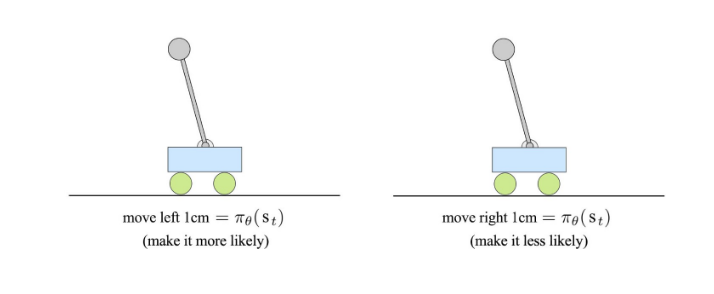
\includegraphics[width=0.7\linewidth]{Figures/RL/RL-cartpole}
%	\caption{}
%	\label{fig:rl-cartpole}
%\end{figure}